% Created 2024-09-23 Mon 13:35
% Intended LaTeX compiler: pdflatex
%%% TeX-command-extra-options: "-shell-escape"
\documentclass[11pt]{article}
\usepackage[utf8]{inputenc}
\usepackage[T1]{fontenc}
\usepackage{graphicx}
\usepackage{longtable}
\usepackage{wrapfig}
\usepackage{rotating}
\usepackage[normalem]{ulem}
\usepackage{amsmath}
\usepackage{amssymb}
\usepackage{capt-of}
\usepackage{hyperref}
\makeatletter
\newcommand{\citeprocitem}[2]{\hyper@linkstart{cite}{citeproc_bib_item_#1}#2\hyper@linkend}
\makeatother
\usepackage[a4paper, total={6in, 8in}]{geometry}
\author{Distributed Lab}
\date{\today}
\title{BitVM fast recap}
\hypersetup{
  pdfauthor={Distributed Lab},
  pdftitle={BitVM fast recap},
  pdfkeywords={},
  pdfsubject={},
  pdfcreator={Emacs 29.4 (Org mode 9.7.11)},
pdflang={English}}
\usepackage{biblatex}

\addbibresource{refs.bib}

\begin{document}

\maketitle

\begin{abstract}
  Assume some user wants to publicly execute a large program on the
  Bitcoin chain using Bitcoin Script, but its implementation is larger
  than 4 megabytes (for example, a Zero Knowledge proof); that is why it
  cannot fit in the transaction input. This document is a fast recap of
  the BitVM2 doc, which proposes optimistic execution verification with
  fraud proofs in case of incorrectness.
\end{abstract}

\setcounter{tocdepth}{2}
\tableofcontents

\section{Introduction}\label{sec:intro}

In the ever-evolving landscape of blockchain technology, the desire to
execute increasingly complex and large-scale programs on the
Bitcoin\autocite{bitcoin_paper} network is growing. However, Bitcoin
Script, the native programming language of Bitcoin, imposes strict
size limits, such as the 4-megabyte cap on transaction inputs, which
makes it challenging to implement certain advanced cryptographic
proofs, like Zero Knowledge proofs. To address this limitation, the
BitVM2\autocite{bitvm2} proposal introduces an innovative approach
that enables the optimistic execution of large programs on the Bitcoin
chain. This method leverages fraud proofs to ensure the validity of
executions, offering a robust mechanism for verifying computations,
while providing a fail-safe against incorrect or malicious
operations. This document provides a concise overview of BitVM2,
highlighting its potential to unlock new possibilities for secure and
scalable program execution on Bitcoin.

\section{Program splitting}\label{sec:program-splitting}

\begin{quote}
  Let there be a large program \(f\), which can be described in Bitcoin
  Script. We want to compute it \textbf{\textbf{on-chain}}, i.e., find
  such an \(f(x) = y\). To achieve this, we divide the program into
  \(n\) sub-programs \(f_1, \ldots, f_n\) and their corresponding
  intermediate states \(z_1, \ldots, z_n\), such that:

  \begin{equation}
    \begin{aligned}
      f_1(x) &= z_1 \\
      f_2(z_1) &= z_2 \\
      &\cdots \\
      f_n(z_{n-1}) &= y
    \end{aligned}
  \end{equation}
\end{quote}

However, the user (referred in BitVM2 as the operator) only needs to
prove that the given program \(f\) indeed returns \(y\) for \(x\), or
\textbf{give others the opportunity disprove this fact}. In our case,
this means giving challengers the ability to prove that at least one
of the sub-programs \(f_i(z_{i-1}) \neq z_i\).

\section{\textbf{Assert} transaction}\label{sec:assert-tx}

To achieve this, the user publishes an \textbf{Assert} transaction,
which has one output with multiple possible spending scenarios:

\begin{enumerate}
  \item \textbf{PayoutScript} (\textbf{LockTime} + signature) --- the
    transaction has passed verification, and the operator can spend the
    output, thereby confirming the statement \(f(x) = y\).
  \item \textbf{DisproveScript} --- one of the challengers has found a
    discrepancy in the intermediate states \(z_i\), \(z_{i-1}\) and the
    sub-program \(f_i\). In other words, they have proven that
    \(f_i(z_{i-1}) \neq z_i\), and thus, they can spend the output.
\end{enumerate}

\subsection{\texttt{DispoveScript}}\label{sec:dispove-script}

\texttt{DispoveScript} is part of the MAST tree in a Taproot address,
which allows challengers to claim the transaction amount for states
\(z_i\), \(z_{i-1}\), and sub-program \(f_i\), is called
\(DisproveScript_i\) in BitVM2:

\begin{verbatim}
// push z_i, z_{i-1} onto the stack
{ z_i     }
{ z_(i-1) }
// compute f(z_{i-1})
{ f_i     }
// ensure that f_i(z_{i-1}) != z_i
OP_EQUAL
OP_NOT
\end{verbatim}

In fact, this script does not need a \texttt{script\_sig}, as with the
correct \(z_i\) and \(z_{i-1}\), it will always execute
successfully. Therefore, to restrict spending capability, a Lamport
signature verification is added to the script.

\subsection{Lamport signature}\label{sec:lamport-signature}

Unlike other digital signature algorithms, the Lamport signature uses
a pair of random secret and public keys \((sk_{\mathcal{M}},
pk_{\mathcal{M}})\) that can sign and verify only any message from the
space \(\mathcal{M} = {\{0, 1\}}^{l}\) of \(\ell\) -bit messages.

However, once the signature \(c_{m}\) is formed, where \(m\) is the message
being signed, \((sk_{\mathcal{M}}, pk_{\mathcal{M}})\) become tied to \(m\),
because any other signature with these keys will compromise the keys
themselves. Thus, for the message \(m\), the keys \((sk_{\mathcal{M}},
pk_{\mathcal{M}})\) are one-time use. From now on, we will denote them as
\((sk_{m}, pk_m)\).

Thus, by taking the intermediate states \(z_i\) as the message for the
Lamport signature, we form one-time key pairs: \((sk_{z_0,
}pk_{z_0})\), \((sk_{z_1, }pk_{z_1})\), \(\ldots\), \((sk_{z_{n-1},
}pk_{z_{n-1}})\) and signatures \(c_{z_1}\), \(\ldots\),
\(c_{z_{n-1}}\), respectivly. Then, to spend the output from the
\texttt{Assert} transaction using the \(DispoveScript_i\) script,
challenger is required adding the corresponding states \(z_i\),
\(z_{i-1}\), and signatures \(c_{z_{i}}\), \(c_{z_{i-1}}\) to the
stack in the \texttt{script\_sig}, making the \texttt{script\_sig} of
the transaction input like this:

\begin{verbatim}
// push z_i, z_{i-1} onto the stack
{ z_i         }
{ z_(i-1)     }
// push c_{z_i}, c_{z_{i-1}} onto the stack
{ c_(z_i)     }
{ c_(z_(i-1)) }
\end{verbatim}

By adding the signatures verification code and public keys to the
\texttt{DisproveScript}s, they become:

\begin{verbatim}
// Push the keys corresponding to states z_i, z_{i-1}
{ pk_(z_i)      }
{ pk_(z_(i-1))  }
// Verify the Lamport signature
{ CheckLampComm }
// compute f(z_{i-1})
{ f_i           }
// ensure that f_i(z_{i-1}) != z_i
OP_EQUAL
OP_NOT
\end{verbatim}

where, as noted in BitVM2, \texttt{CheckLampComm} (or
\texttt{Lamport.Vrfy}) is the verification of the Lamport signature
(commitment), described in Bitcoin Script (as Bitcoin Script does not
have a built-in ``opcode'' for Lamport signatures).

However, in newer implementations, it has been proposed to use the
Winternitz signature, which has the same properties but requires fewer
``opcodes''.

\subsection{Structure of the MAST Tree in a Taproot
Address}\label{sec:mast-tree-structure}

The inputs of the \texttt{Assert} transaction spend the output to a
Taproot address, which consists of a MAST tree of Bitcoin scripts
mentioned in Section~\ref{sec:assert-tx}. From the BitVM2 document, it
is known that the first \(n\) scripts in the tree are all
\(DisproveScript_i\), where \(i = \overline{1, n}\), and the last is a
script that allows the operator who published the \texttt{Assert}
transaction to spend the output after some time. A visualization of
this tree can be seen in the figure~\ref{fig:assert-tx-mast-tree}.

\begin{figure}[htbp]
  \centering
  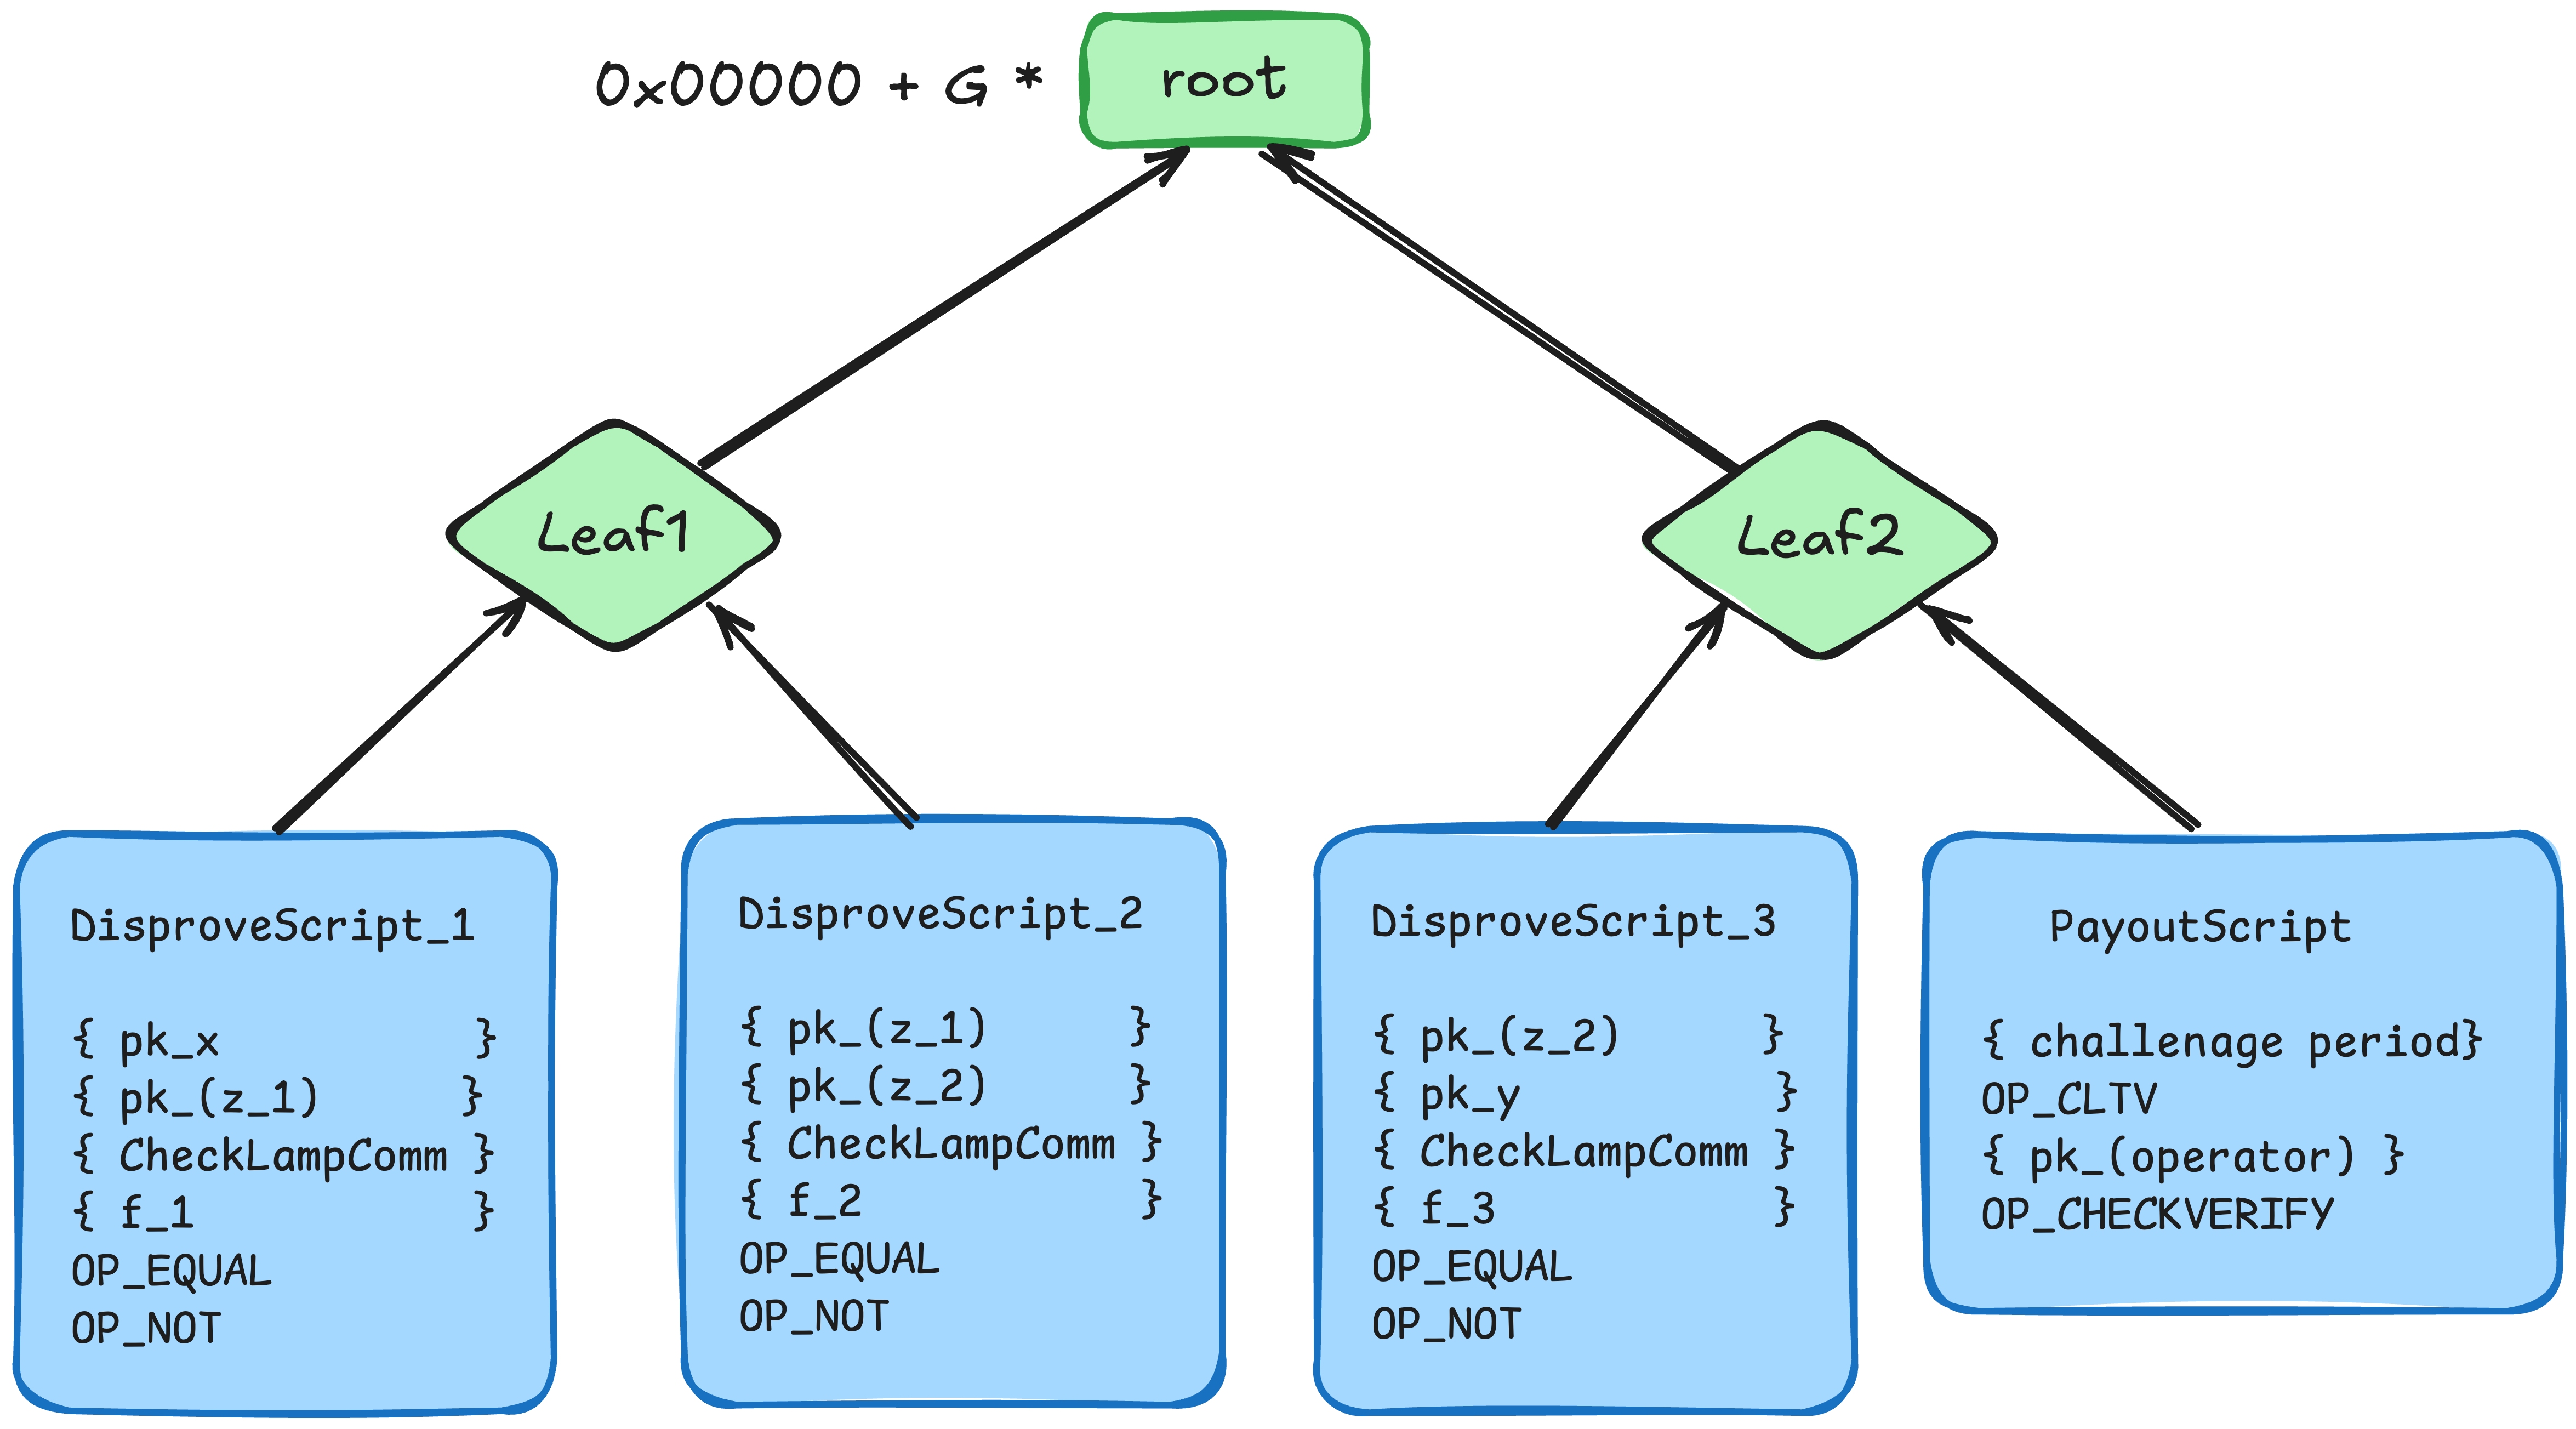
\includegraphics[width=.9\linewidth]{../images/assert-tx-taproot-output.png}
  \caption{\label{fig:assert-tx-mast-tree}Script tree in a Taproot
  address with three sub-programs and two intermediate states.}
\end{figure}

\section{\texttt{Disprove} and \texttt{Payout}
transactions}\label{sec:disprove-payout-txs}

These are transactions that spend the output from \texttt{Assert} via
\texttt{DisproveScript} and \texttt{PayoutScript} respectively (see
fig.~\ref{fig:bitvm-txs}). Their structure becomes more important when
we consider the emulation of ``covenants'' through a committee.

\begin{figure}[htbp]
  \centering
  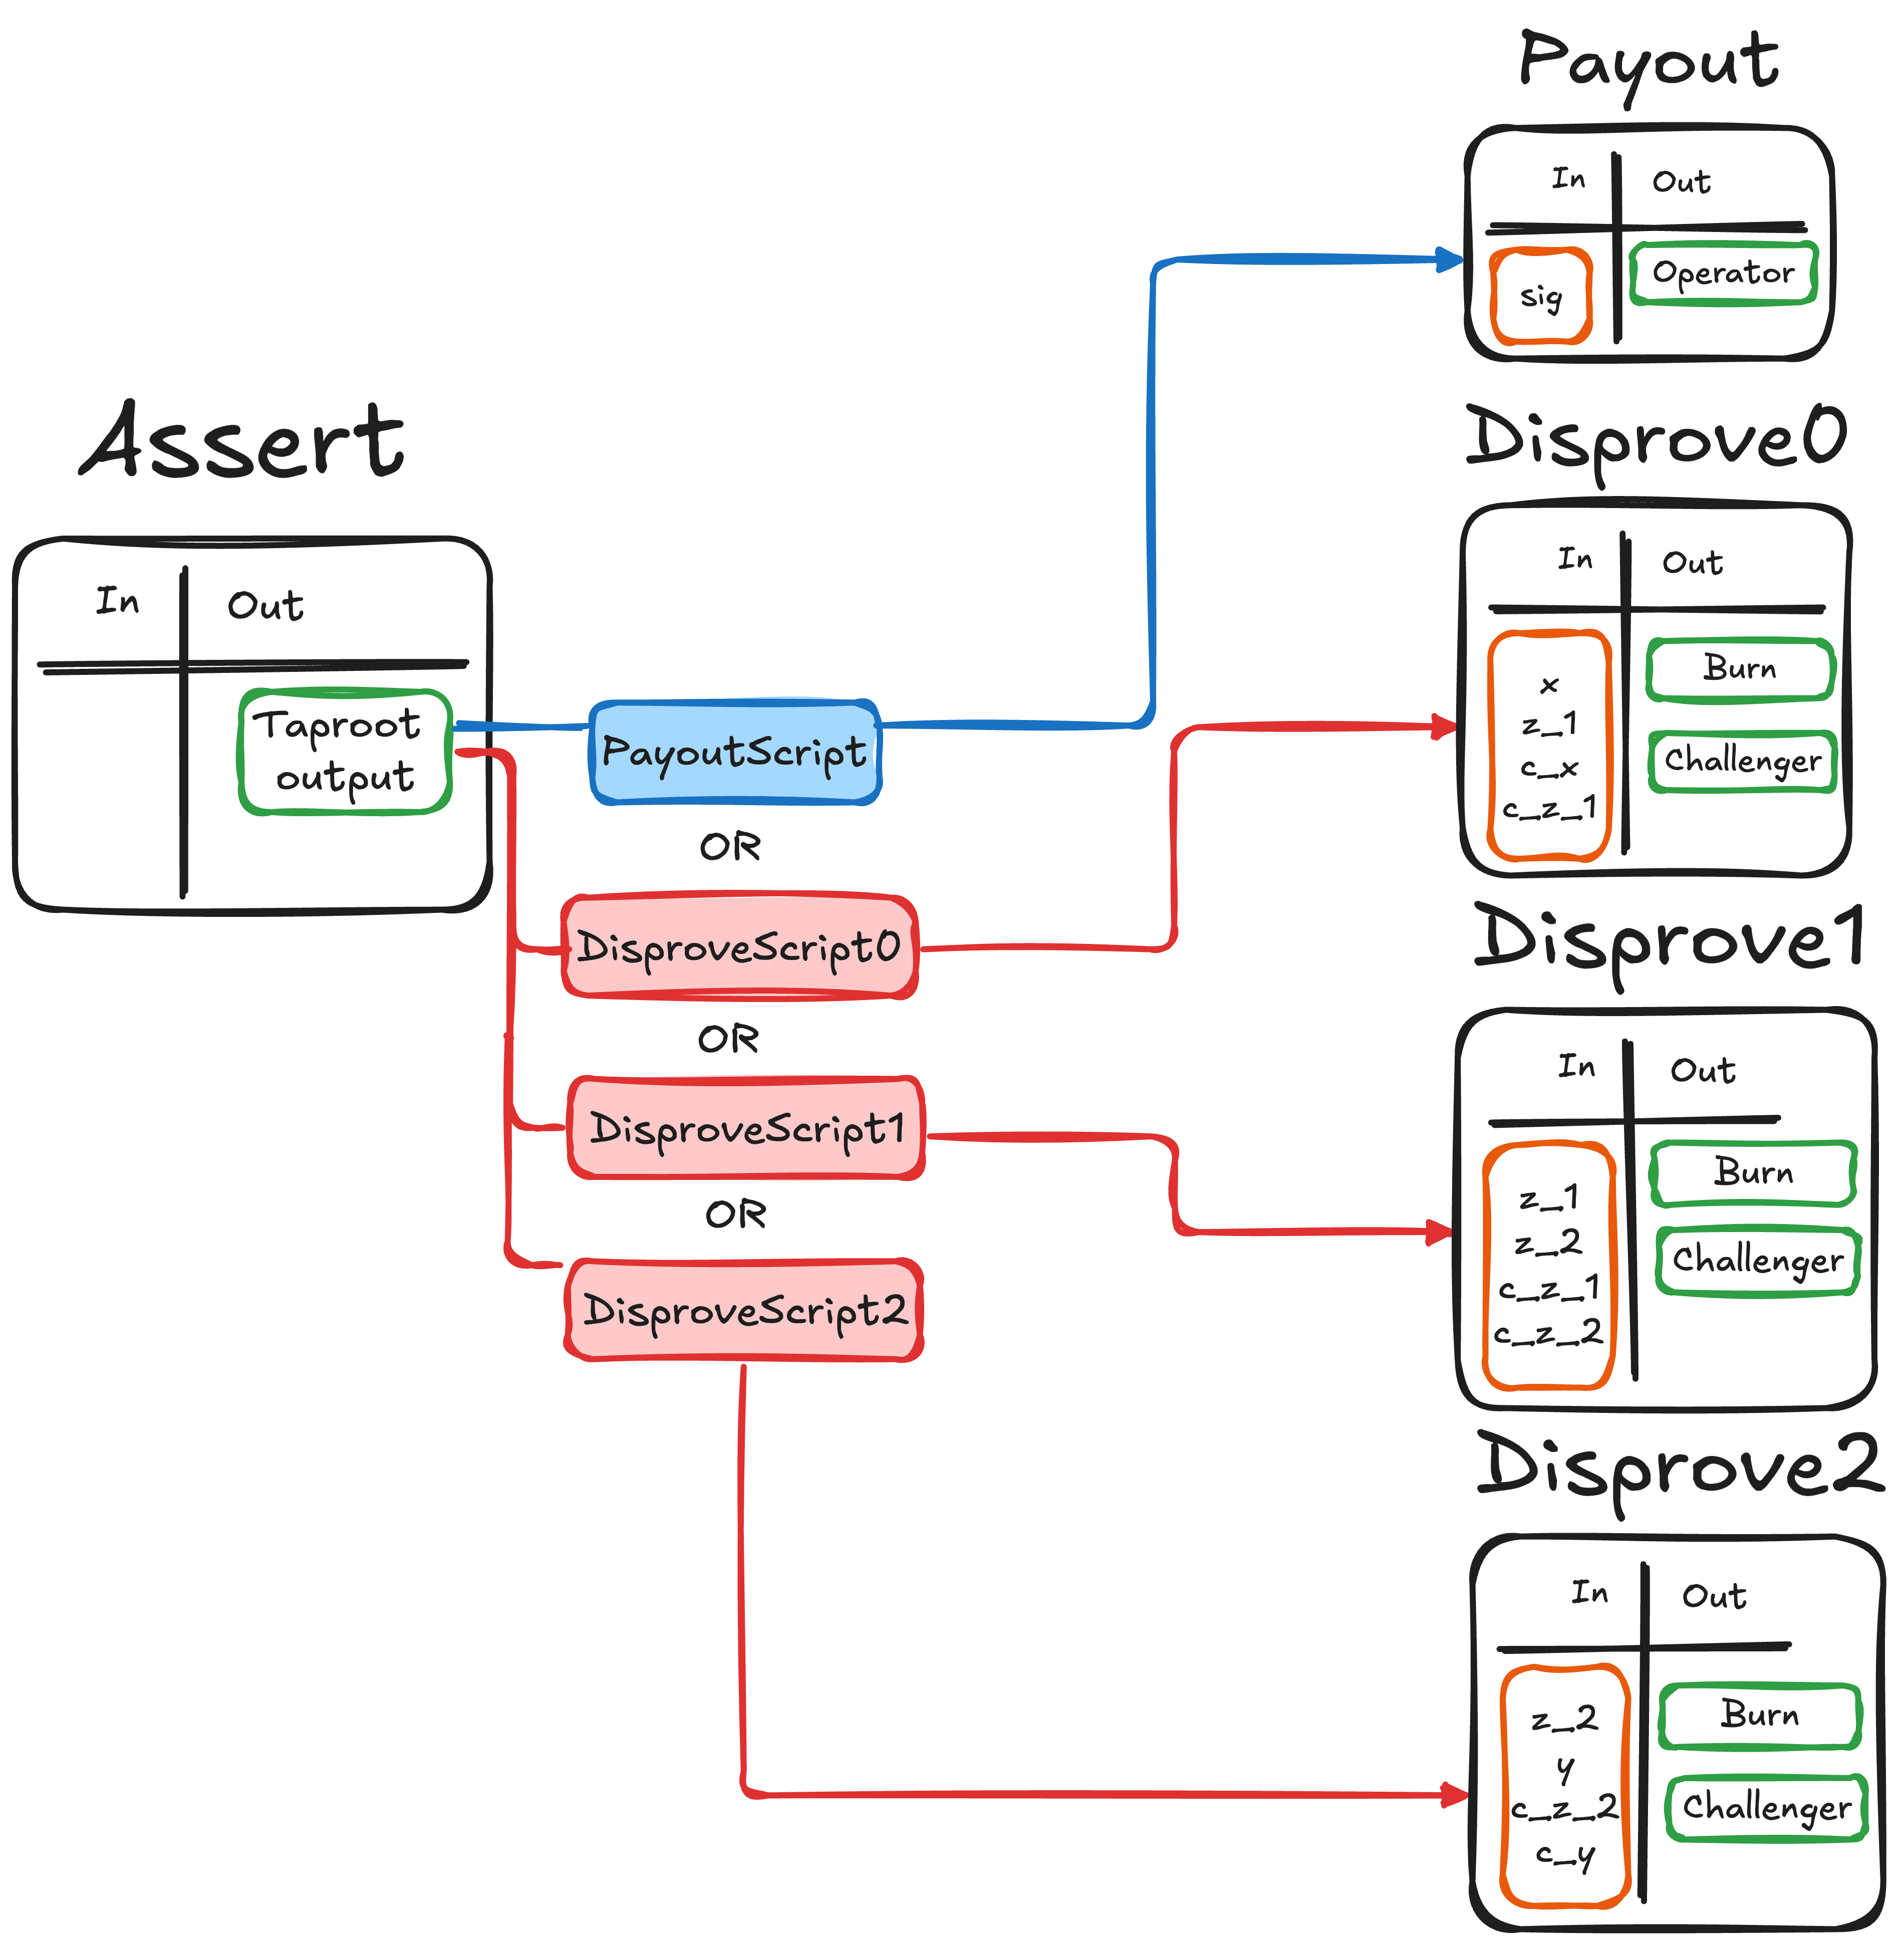
\includegraphics[width=.9\linewidth]{../images/bitvm-txs.png}
  \caption{\label{fig:bitvm-txs}Sequance of transactions in BitVM2
  with 3 subprograms and 2 intermediate states.}
\end{figure}

\section{{\bfseries\sffamily TODO} Covenants emulation through
comittee}\label{sec:covenants-emulation}

\printbibliography{}

\end{document}
